% ---------------------------------------------------------------------
% ---------------------------------------------------------------------
% ---------------------------------------------------------------------
\part{Materials and methods}

\chapter[Multiway data, methods for its analysis]{Multiway data, methods for its analysis}
\label{chapter:threeways}


% ---------------------------------------------------------------------
% ---------------------------------------------------------------------
\section{From 2D matrices to 3D arrays}
In most fields, data sets are usually represented by two dimensional matrices, where the rows are the observations and the columns are the different variables ($I \times J$). But in metabolomics, and in general in many other 'omic' sciences, sometimes these $I \times J$ data sets can be expanded by taking, for example, repeated measurements at different $K$ time points for each observation and producing a three-dimensional data structure ($I \times J \times K$) called three-way array (\autoref{figura27}) or, more generally, a multidimensional data structure called multi-way array \parencite{kroonenberg2016my}. Most of the modelling methods that have been explained in \autoref{chapter:modern_techniques} are not able of dealing with such data structures, which raise many methodological complications to the analyses. Therefore, different three-way or multi-way specific methods have been developed during the last decades to deal with this sort of data.

\begin{figure}[hbtp]
\centering
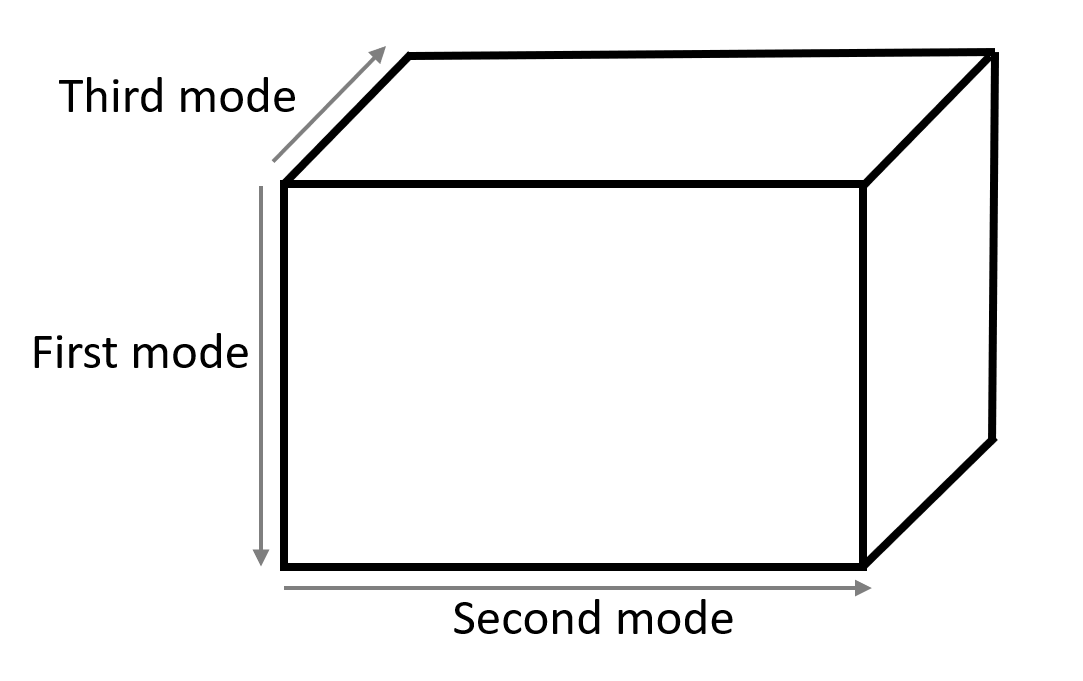
\includegraphics[width=0.60\textwidth]{figura27.png}
\caption{Representation of a three-way array.}
\label{figura27}
\end{figure}

\section{Exploration and description of N-way arrays}
\subsection{Unfolding}
One of the straightforward solutions for dealing with $N$-way arrays is performing an unfolding of the array into a two-dimensional matrix. This unfolding is performed by regrouping the elements of the higher order dimensions, also called modes, by extending the dimension of the second mode, as showed in \autoref{figura35}. After the unfolding, all statistical methods valid for two-dimensional matrices are applicable to the new structure, although the tridimensional structure of the data is lost, leading to a list of potential issues such as more complex models (too many parameters), loss of predictive power, loss of the multi-way information and greater difficulty in the interpretation of results.

\begin{figure}[hbtp]
\centering
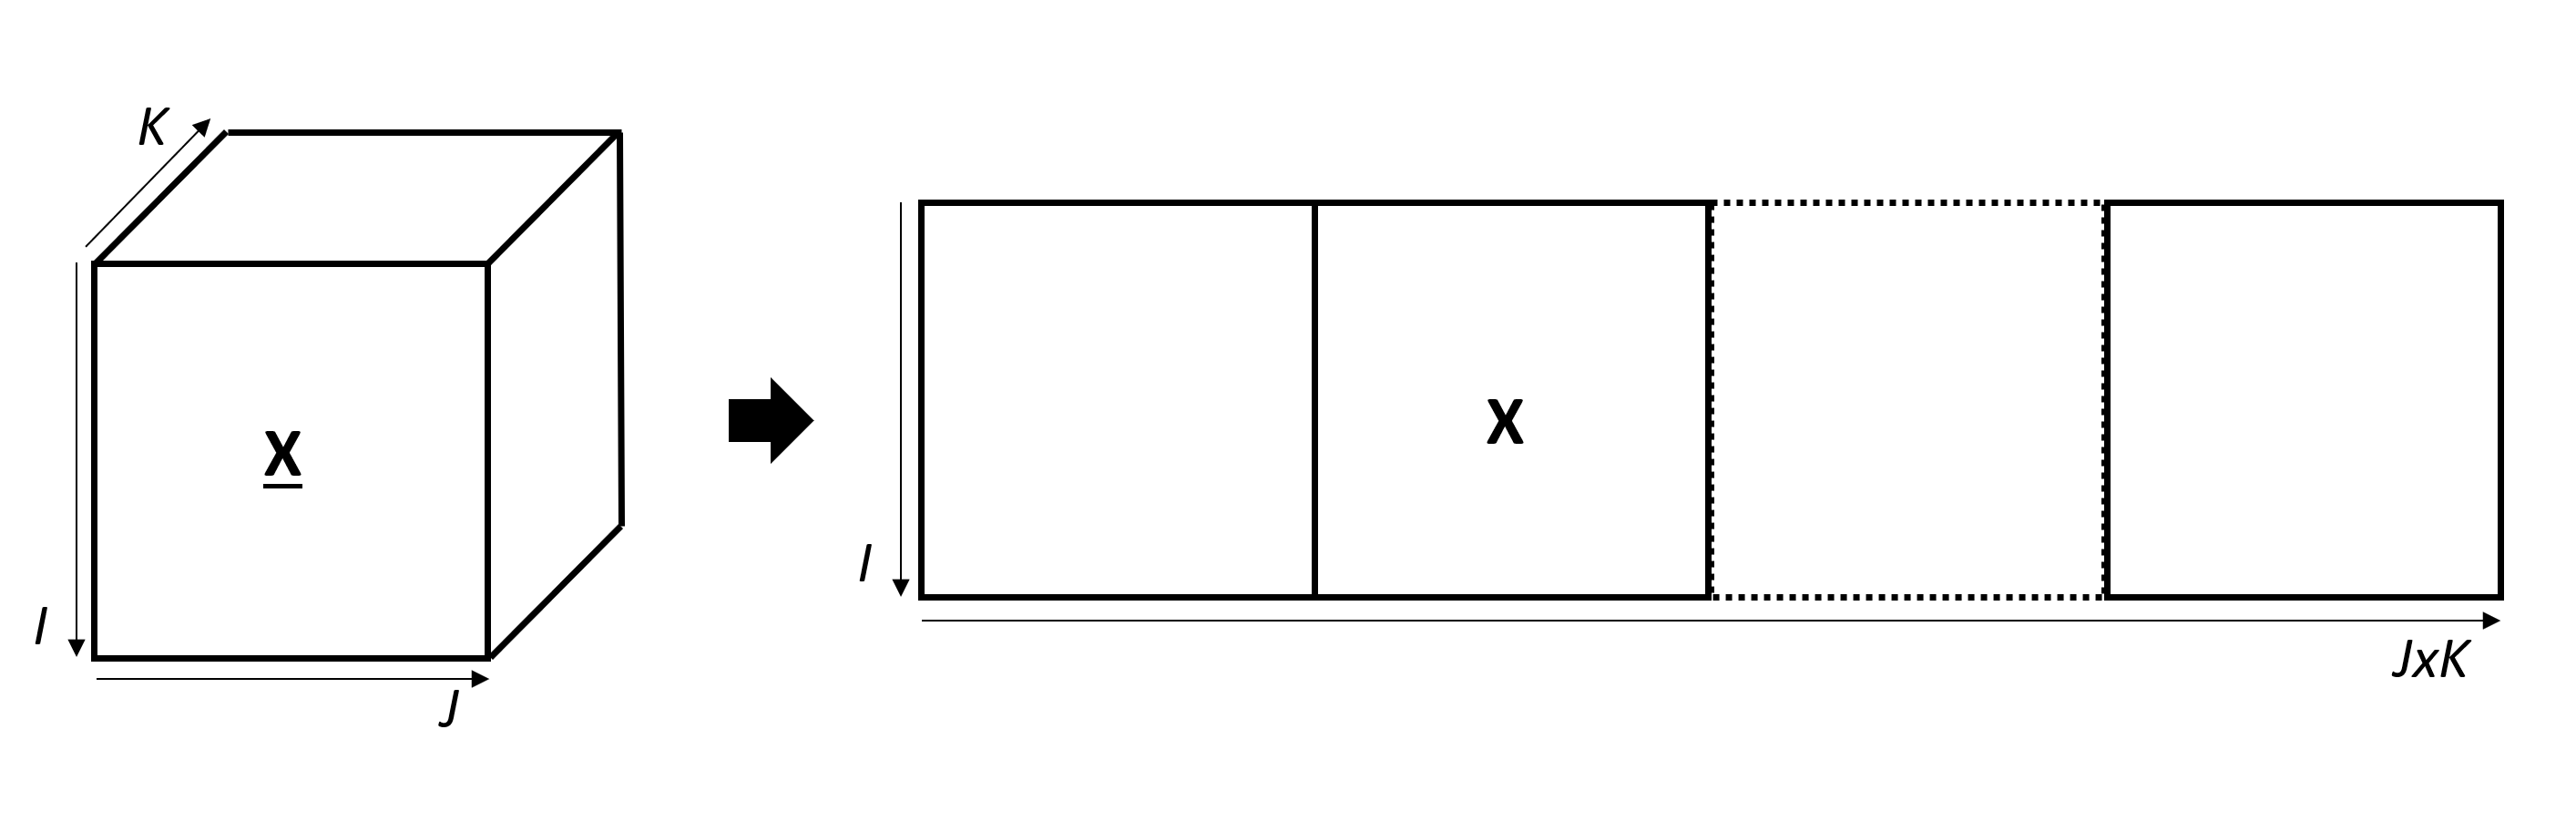
\includegraphics[width=0.95\textwidth]{figura35.png}
\caption[Unfolding of a three-way array into a two-dimensional matrix]{Unfolding of a three-way array ($I \times J \times K$) into a two-dimensional matrix ($I \times JK$).}
\label{figura35}
\end{figure}


\subsection{Tucker3}
When studying multi-way structures, the most general model that can be used is the Tucker3 model \parencite{tucker1966some}, also explained in detail by \textcite{kiers2001three}.

Assuming a three-way structure of the data, the Tucker3 model has the structure defined in \autoref{figura34}. This figure shows that the model is a weighted sum of all possible outer products, where the weights of the outer product between the $i$th factor from \textbf{A}, the $j$th factor from \textbf{B} and the $k$th factor from \textbf{C} is determined by element $g_{ijk}$ of the core. 

Model parameters are estimated by minimizing the squared sum of residuals $e_{lmn}$ as shown in \autoref{equation17}

\begin{equation}
x_{ijk}=\sum\limits_{l=1}^{w_1} \sum\limits_{m=1}^{w_2} \sum\limits_{n=1}^{w_3}a_{il}b_{jm}c_{kn}+e_{lmn}
\label{equation17}
\end{equation}

If the Kronecker product is used, defined as $\otimes$, unfolding the \textbf{\underline{X}} array, the \textbf{\underline{G}} core and the residuals \textbf{\underline{E}} into matrices \textbf{X}, \textbf{G} and \textbf{E} by fixing the first mode, the matrix expression of the model is as follows (\autoref{equation18}):

\begin{equation}
\textbf{\text{X}}=\textbf{\text{AG}}(\textbf{\text{C}}^T\otimes \textbf{\text{B}}^T)+\textbf{\text{E}}
\label{equation18}
\end{equation}

where \textbf{A} is the loadings matrix corresponding to the first mode, \textbf{G} is the matrix obtained after unfolding the \textbf{\underline{G}} core fixing the first mode, \textbf{B} and \textbf{C} are the loading matrices of the second and third mode respectively and \textbf{E} is the residuals matrix. The fact that the number of components is not forced to be the same in the different modes allows for the different loadings matrices to have different dimensions for each mode.

\begin{figure}[hbtp]
\centering
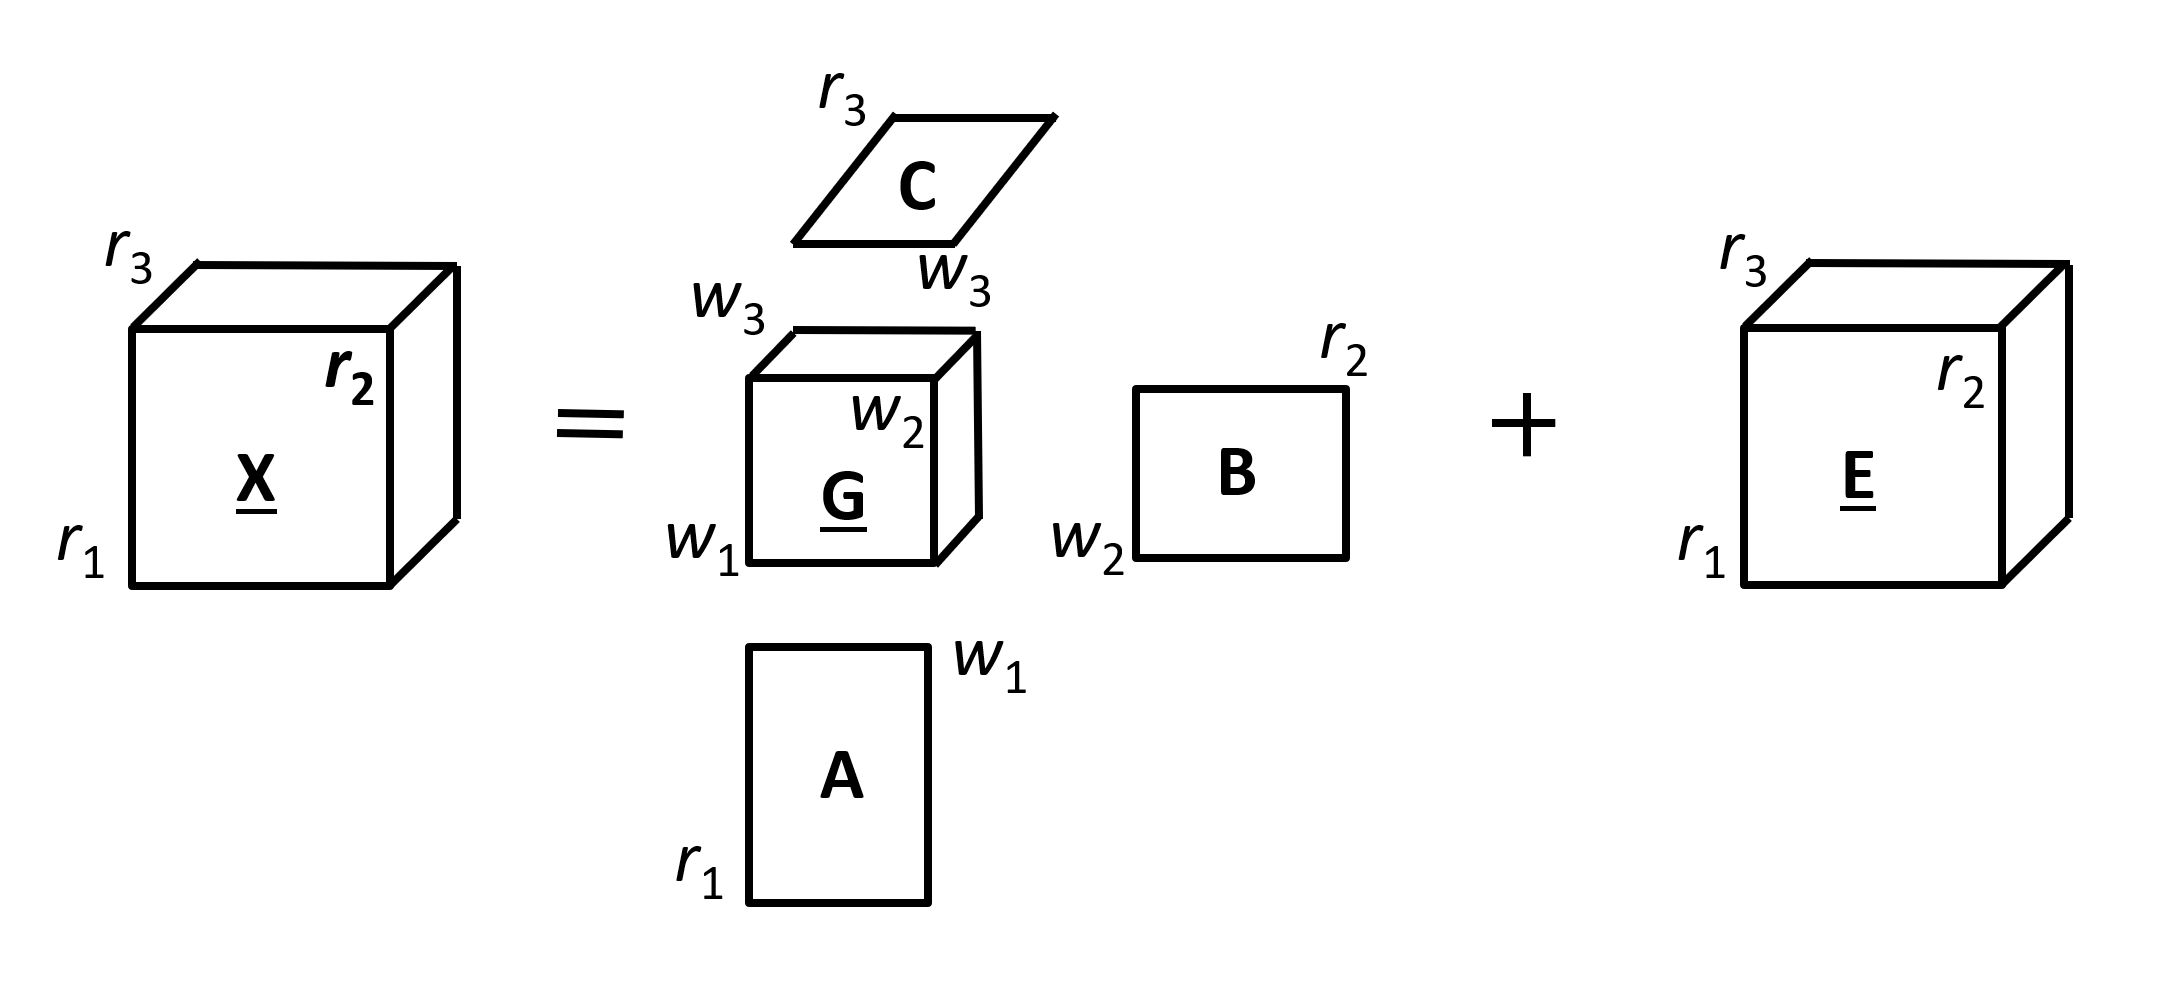
\includegraphics[width=0.85\textwidth]{figura34.png}
\caption[Scheme of the Tucker3 model]{Scheme of the Tucker3 model. The model consists on a weighted sum of outer products between the different factors stored in matrices \textbf{A}, \textbf{B} and \textbf{C}.}
\label{figura34}
\end{figure}

Of note, the compression performed by the model can be applied also to the first mode. This way, the \textbf{\underline{G}} core can be considered as an approximation to \textbf{\underline{X}}, which approximates the original array by the three matrices \textbf{A}, \textbf{B} and \textbf{C}.

It is important to take into account that the model has not a unique solution, because it has rotational freedom. In fact, the model can be so redundant that many elements of \textbf{\underline{G}} can be set to zero without altering the fit of the model, thus meaning they are associated to noise \parencite{montalban2005control}.

\subsection{PARAFAC}
The PARAFAC method is also a decomposition method for multi-way arrays. It can be derived from the Tucker 3 model by imposing superdiagonallity and identity in the structure of the \textbf{\underline{G}} core. Essentially, it is a generalization of PCA to three- or multi-way data structures \parencite{bro1997parafac}. The method was first developed by \textcite{harshman1970foundations} and \textcite{carroll1970analysis}, who named the method as CANDECOMP. In this method, the decomposition of the data is made into trilinear components, with each component consisting of one score vector and two loading vectors. The general structure of the PARAFAC model is presented in \autoref{figura36}.

\begin{figure}[hbtp]
\centering
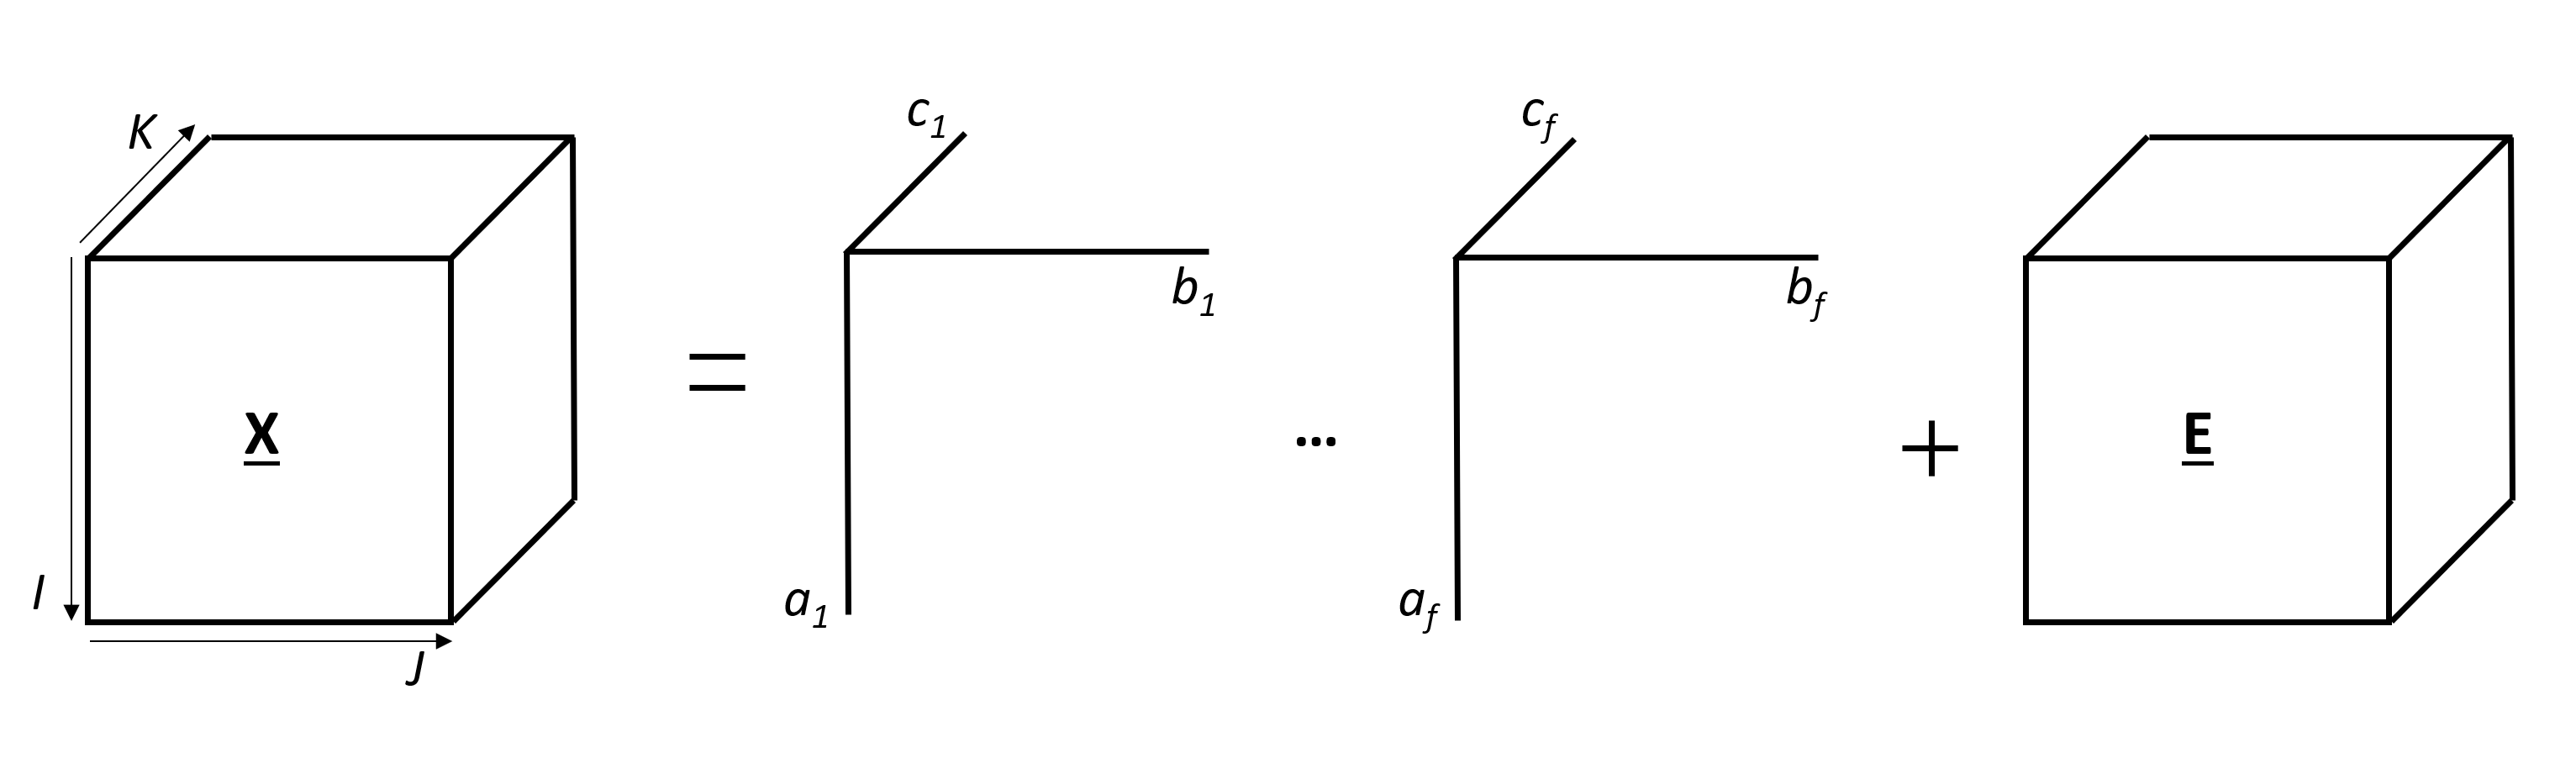
\includegraphics[width=0.9\textwidth]{figura36.png}
\caption{General structure of a PARAFAC model.}
\label{figura36}
\end{figure}

A PARAFAC model of a three-way array is given by three loading matrices, \textbf{A}, \textbf{B} and \textbf{C} with elements $a_{if}$, $b_{if}$ and $c_{kf}$. The model minimizes the sum of squares of residuals in \autoref{equation16}.

\begin{equation}
x_{ijk}=\sum\limits_{f=1}^F a_{ij}b_{jf}c_{kf}+e_{ijk}
\label{equation16}
\end{equation}

The matricial expression of the PARAFAC model can be obtained by Using the Khatri-Rao product \parencite{liu2008hadamard} and by unfolding the \textbf{\underline{X}} array into matrix \textbf{X} (\autoref{equation19}).

\begin{equation}
\textbf{\text{X}}=\textbf{\text{A}}(\textbf{\text{C}}|\otimes|\textbf{\text{B}})^T + \textbf{\text{E}} = \sum\limits_{f=1}^F a_f(c^T_f\otimes b^T_f)+\textbf{\text{E}}
\label{equation19}
\end{equation}

In the PARAFAC model, $a_f$, $b_f$ and $c_f$ are the $f$th columns of the loading matrices \textbf{A}, \textbf{B} and \textbf{C}, respectively.

The main advantage of PARAFAC over Tucker3 models is the impossibility of alternative solutions, that is, there is no posibility of rotation. This makes PARAFAC models more easily interpretable.

\section{Regression methods for \textit{N}-way arrays, \textit{N}-PLS}
\label{NPLSregression}
The $N$-PLS model is an extension of the standard PLS model to multi-way arrays based in the decomposition performed by the PARAFAC model \parencite{bro1996multiway}. Its aim is studying relationships between some three-way (or N-way) \textbf{\underline{X}} (e.g. $I \times J \times K$) data structure and any \textbf{\underline{Y}} (e.g. $I \times L \times M$) data structure by maximizing the covariance between \textbf{\underline{X}} and \textbf{\underline{Y}} data arrays. For achieving this, a multilinear model is fitted simultaneously to the \textbf{\underline{X}} and the \textbf{\underline{Y}} arrays with a regression model relating them together. The structure of the $N$-PLS model is presented in \autoref{figura38}.

\begin{figure}[hbtp]
\centering
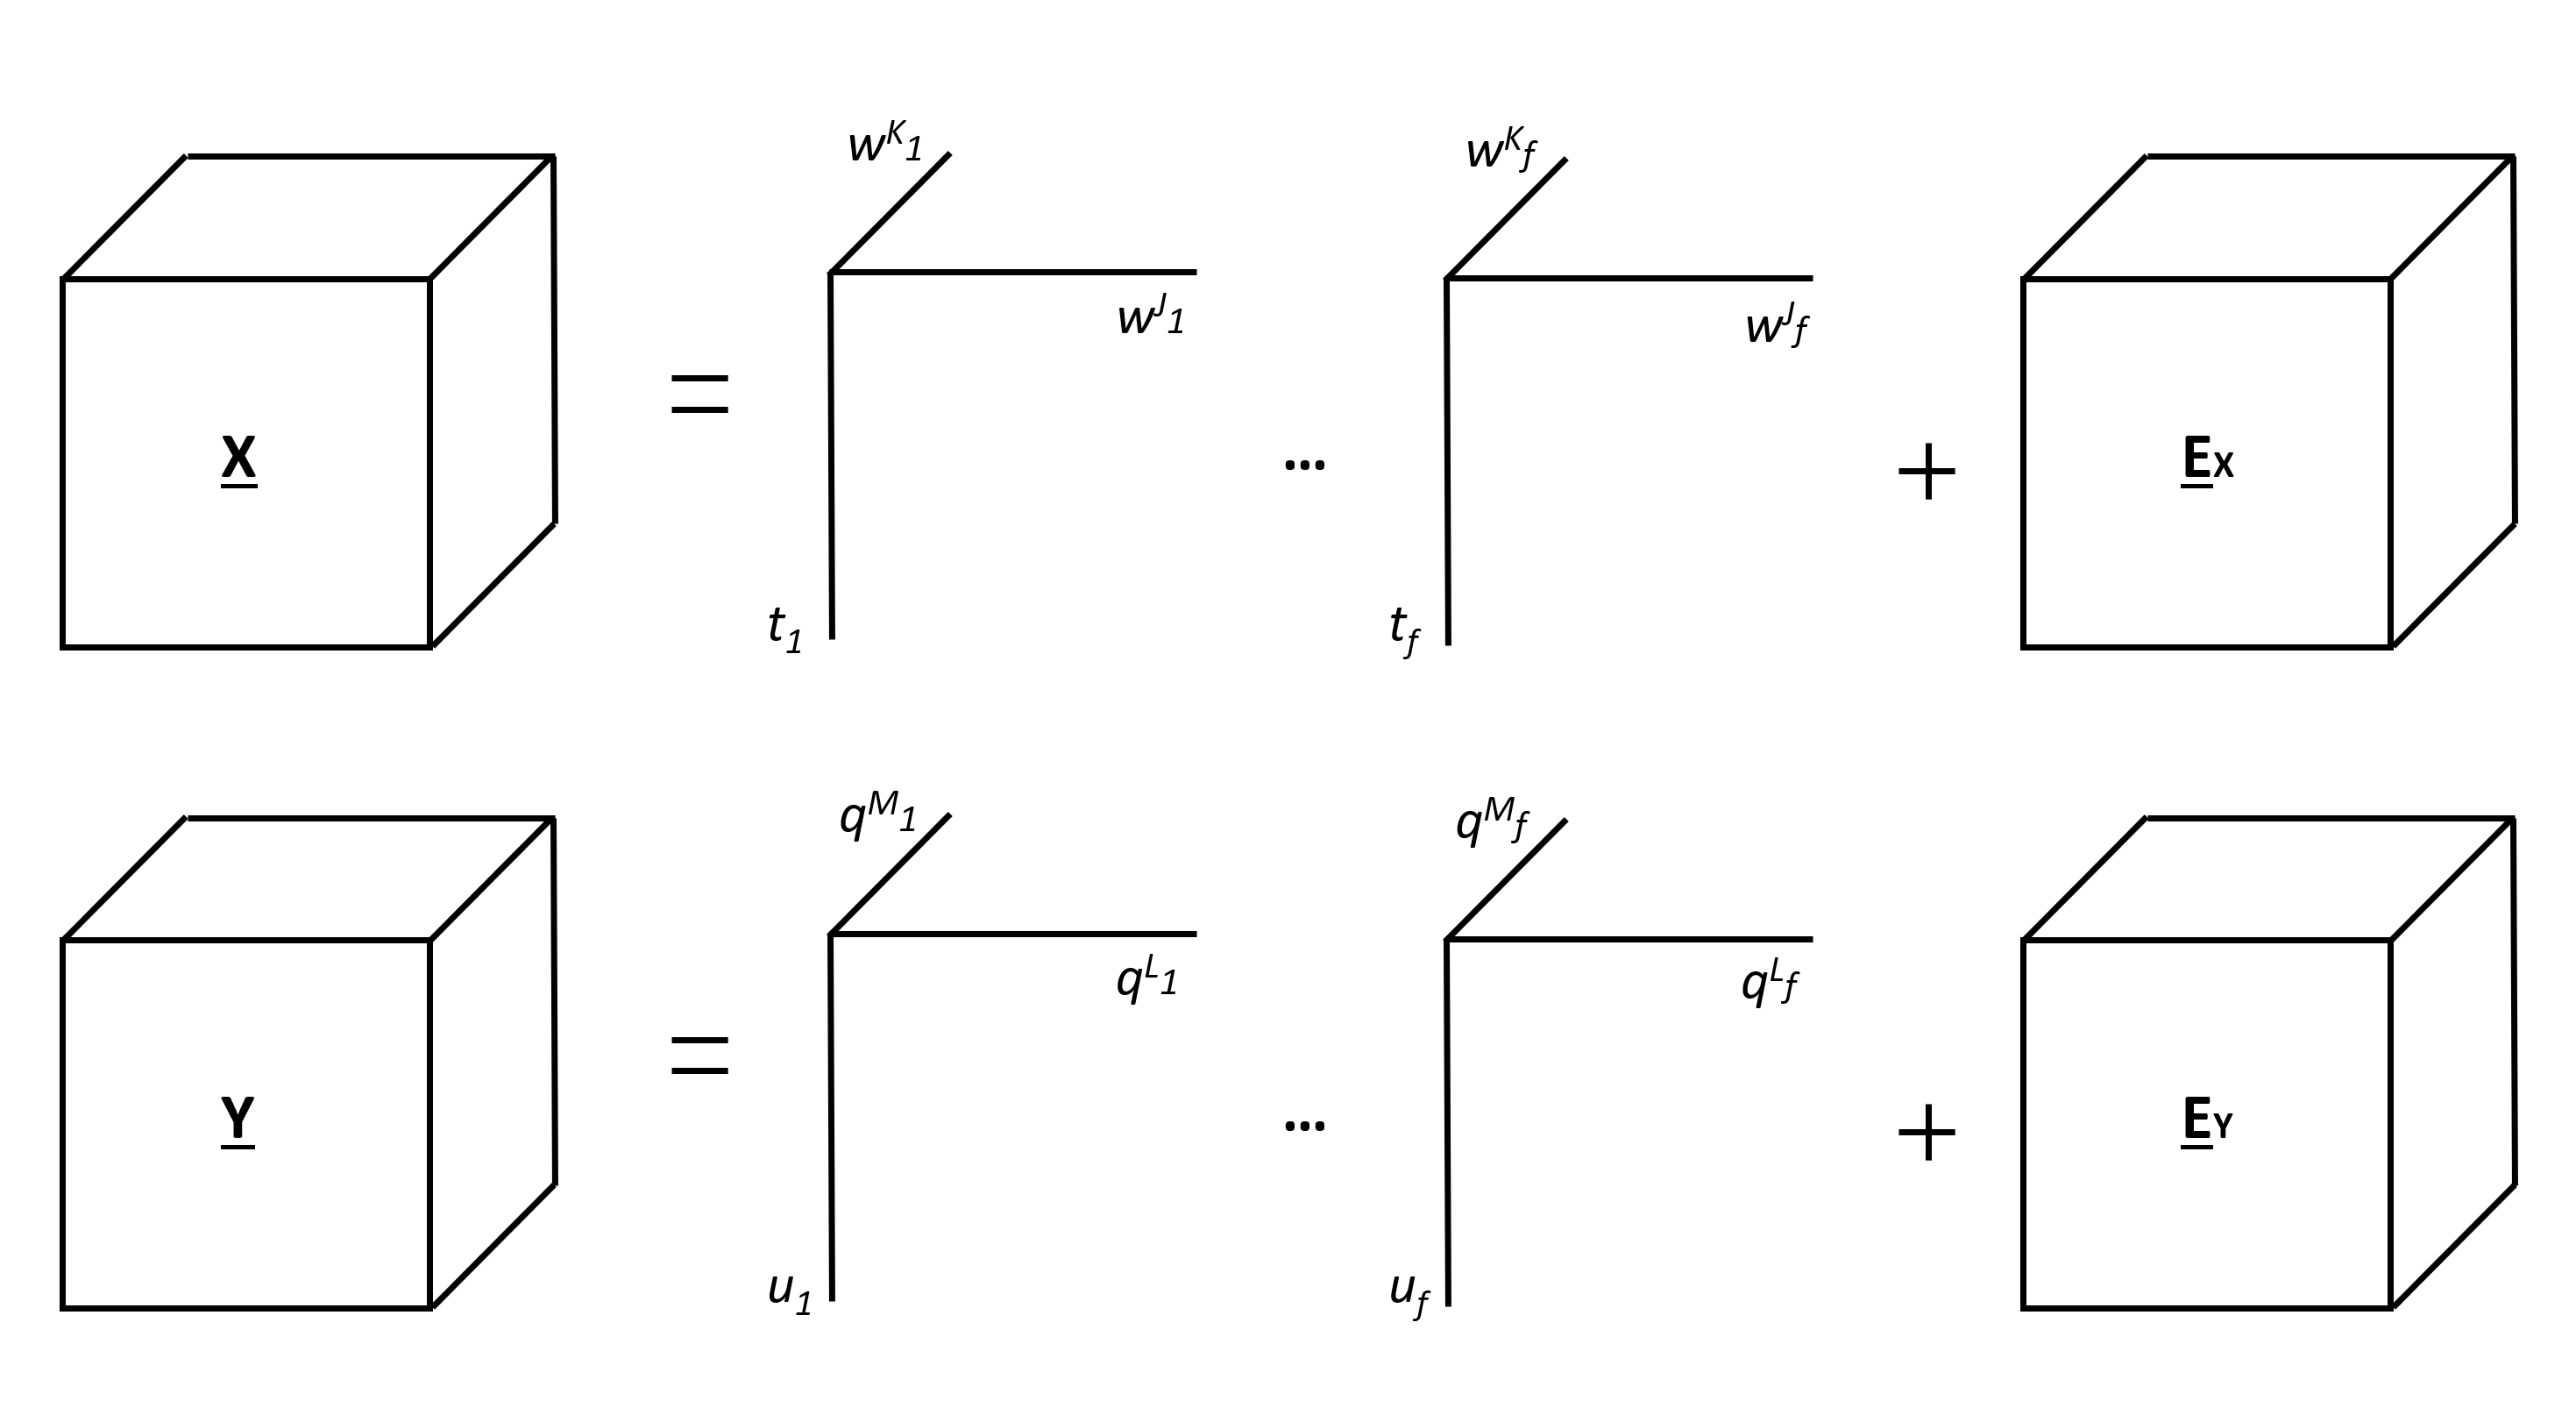
\includegraphics[width=0.85\textwidth]{figura38.png}
\caption{General structure of a $N$-PLS model.}
\label{figura38}
\end{figure}


Considering \textbf{X} ($I \times JK$) the unfolded version of \textbf{\underline{X}}, \textit{N}-PLS tries to find latent spaces $\textbf{\text{W}}^{J}$ and $\textbf{\text{W}}^{K}$ that maximize the covariance between \textbf{X} and \textbf{Y}, so it can be expressed as:

\begin{equation}
\textbf{\text{X}}=\textbf{\text{T}}(\textbf{\text{W}}^{K}|\otimes{}|\textbf{\text{W}}^{J})^{T}+\textbf{\text{R}}
\label{equation01}
\end{equation}

Afterwards decomposing \textbf{\underline{X}} from \textbf{X} using the improved $N$-PLS version expression \parencite{bro2001difference}, in order to obtain residuals with better statistical properties:

\begin{equation}
\textbf{\text{X}}=\textbf{\text{T}}\textbf{\text{Gu}}(\textbf{\text{W}}^{K}\otimes{}\textbf{\text{W}}^{J})^{T}+\textbf{\text{R}}^{\boldsymbol{\prime{}}}
\label{equation02}
\end{equation}

In the same way, \textbf{\underline{Y}} can be decomposed by unfolding \textbf{\underline{Y}} ($I \times L \times M$) into \textbf{Y} ($I \times LM$) as:

\begin{equation}
\textbf{\text{Y}}=\textbf{\text{U}}(\textbf{\text{Q}}^{M}|\otimes{}|\textbf{\text{Q}}^{L})^{T}+\textbf{\text{R}}^{\boldsymbol{\prime{}\prime{}}}
\label{equation03}
\end{equation}

In this case, $\textbf{\text{W}}^{K}$ and $\textbf{\text{W}}^{J}$ refer to the weights of the third and of the second mode, respectively; whereas $\textbf{\text{T}}$ matrix gathers the scores of the samples at each component extracted, in the first mode. $|\otimes{}|$ is the Khatri-Rao product and $\otimes{}$ the Kronecker product, which forbid or allow (respectively) to take interactions between the different modes components into account. 
\textbf{Gu} is the core array (unfolded) of a Tucker3 decomposition when using \textbf{T}, $\textbf{\text{W}}^{K}$ and $\textbf{\text{W}}^{J}$ as loadings, in order to obtain a better (or at least not worse) approximation of the \textbf{\underline{X}} array \parencite{smilde2005multi}. Finally, $\textbf{\text{R}}^{\boldsymbol{\prime{}}}$ incorporates the residuals. Analogously, \textbf{U} refers to the \textbf{Y} scores, and $\textbf{\text{Q}}^{M}$ and $\textbf{\text{Q}}^{L}$ to the loadings of the array \textbf{\underline{Y}}.
Finally, from the scores \textbf{T} and \textbf{U}, as well from the \textbf{W} weights, a $\textbf{\text{B}}_{PLS}$ regression matrix can be obtained \parencite{bro1998multi} so

\begin{equation}
\textbf{\text{Y}}=\textbf{\text{X}}\textbf{\text{B}}_{PLS}+\textbf{\text{R}}^{\boldsymbol{\prime{}\prime{}\prime{}}}
\label{equation04}
\end{equation}

In summary, $N$-PLS allows for the application of the well known standard PLS model to multi-way arrays, being able to exploit the multidimensional structure of the data, reducing the inclusion of noise, and producing more parsimonious models than standard PLS models applied to unfolded matrices. 


\section{Software for analyzing three-way data}
\subsection{\texttt{R} programming language}
\texttt{R} \parencite{ihaka1996r, rsoftware} is a programming language designed for statistical programming, derived from the \texttt{S} language, which was developed in the Bell Laboratories by Rick Becker, John Chambers and Allan Wilks in the 60s. It is free software and open source, and was designed specifically for performing data analysis and statistical tasks. Since it is open source, \texttt{R} has thousands of developers, which results in more than 10000 packages in the main software repository for \texttt{R} named \textit{CRAN} (\autoref{figura13}) and more than 1300 packages in the \textit{Bioconductor} repository, specialized in packages for the analysis of 'omic' data. For this reasons, \texttt{R} has become a standard for data analysis in many scientific fields such as physics, biology and medicine among others \parencite{goztepe4facto}. 

\begin{figure}[hbtp]
	\centering
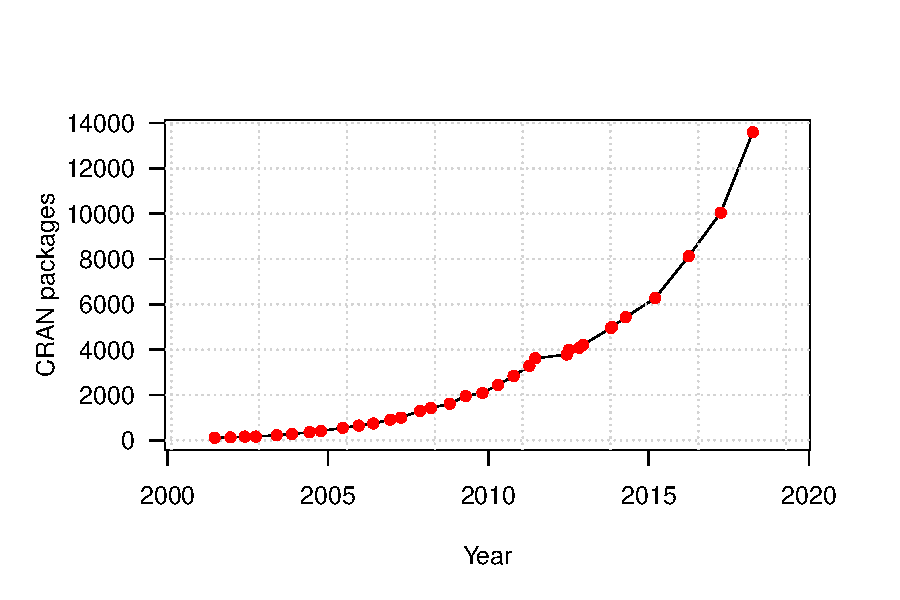
\includegraphics[width=0.7\textwidth]{figura13.pdf}
\caption[Number of R packages on CRAN since 2002]{Number of R packages on CRAN has been growing at an exponential rate since 2002.}
\label{figura13}
\end{figure}

With the huge number of packages at the disposal of \texttt{R} users, many advanced functions have already been programmed and are available for their use or reuse when programming new functionalities. Apart from the main repository (CRAN) there are other important repositories with thousands of packages more such as \textit{R-Forge}, \textit{Bioconductor} or even \textit{Github}. All this functionallity and the fact that R is open source motivated the election of \texttt{R} as the language for developing all the techniques and tools presented in this thesis.

\subsection{\texttt{R} packages for the analysis of three-way data}
Most three-way data procedures are implemented in MATLAB\textsuperscript{\tiny\textregistered} \textcite{MATLAB:2010} (or previous versions of the software). Concretely, the $N$-way toolbox by \textcite{andersson2000n} provides a comprehensive set of functions for dealing with three- and multi-way arrays in MATLAB\textsuperscript{\tiny\textregistered}. \texttt{R}, on the other hand, only has two packages dedicated to the analysis of three- or multi-way data. The packages \texttt{PTAk} \parencite{leibovici2010spatio} and \texttt{ThreeWay} \parencite{giordani2014three}, offer a suit of functions for handling three-way arrays in \texttt{R}. These functions include Tucker3 and PARAFAC models and also some processing methods for three-way data such as centering, scaling, unfolding and normalizing arrays. However, $N$-PLS is notably missing from these packages, so no prediction method for three-way arrays was implemented in \texttt{R} before the release of the \texttt{sNPLS} package developed in this thesis. In this way, with the development of the package, it has not only been implemented a newly developed method such as sparse $N$-PLS, but also enabled the use of standard $N$-PLS regression models to \texttt{R} users.